\documentclass[11pt]{article}

\usepackage[T1]{fontenc}
\usepackage[utf8]{inputenc}
\usepackage[english]{babel}
\usepackage{xspace}
\usepackage{parskip}
\usepackage{amsmath}
\usepackage{amsfonts}
\usepackage{amssymb}
\usepackage{enumitem}
\usepackage[dvipsnames]{xcolor}
\usepackage{graphicx}
\usepackage{subcaption}
\usepackage{booktabs}
\usepackage{float}
\usepackage{array}
\usepackage[
    paper = a4paper,
    margin = 2.5cm,
    top = 2cm,
    bottom = 2cm
]{geometry}
\usepackage[colorlinks = true]{hyperref}
\usepackage{ilatex}


%%%%%%%%%%%%%%%%%%%%%%%%%%%%%%%%%%%%%%%%%%%%%%%%%%%%%

\newcommand{\iLaTeX}{i\LaTeX{}\xspace}

\title{A test file for \iLaTeX}
\author{Camille Gobert (\url{camille.gobert@ens.fr})}
\date{\today}

\linespread{1.05}


%%%%%%%%%%%%%%%%%%%%%%%%%%%%%%%%%%%%%%%%%%%%%%%%%%%%%

\begin{document}
    % Title
    \maketitle
    
    % Body
    Lorem ipsum dolor sit amet.
    Text \emph{accentu\'e} should be supported.
    
    \textbf{This is bold text.}
    \textit{This is italic text.}
    
    This is a \href{https://www.lri.fr/}{hyperlink} to LRI's website.
    
    % Example of some maths
    \paragraph{}
    Inline maths such as $x^2$ are supported, as well as 
    $$e^{i\pi} + 1 = 0$$
    
    % Example of a table
    \begin{table}[h]
        \centering
        \ilatex{\begin{tabular}{lrrr}
            \toprule
            \textbf{Value 1} & \textbf{Value 2} & \textbf{Value 3}  & \textbf{Symbol} \\
            \midrule
            1 & 2 & 3 & $x$ \\
            4 & 5 & 6 & $y$ \\
            7 & 8 & 9 & $z$ \\
            \bottomrule
        \end{tabular}}
        \caption{Random table.}
        \label{tab:random}
    \end{table}

    % Example of a figure
    \begin{figure}[h]
        \centering
        \ilatex{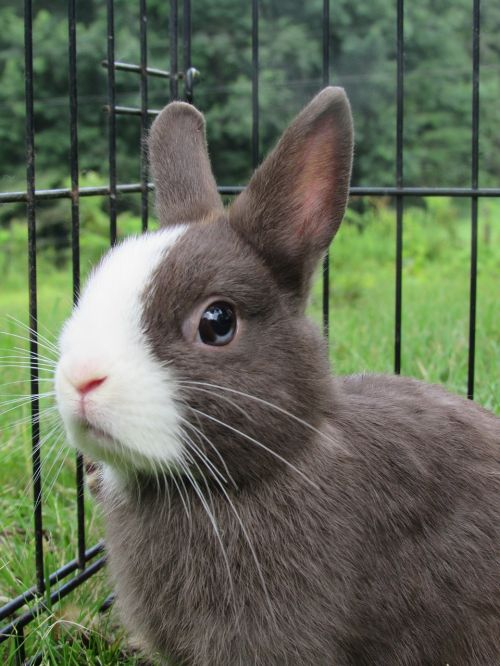
\includegraphics[width=194px, height=255px, trim=15px 147px 109px 50px, clip]{img/rabbit.jpg}}
        \caption{Picture of a rabbit.}
        \label{fig:rabbit}
    \end{figure}

    \newpage
    This text should appear on the second page.

    % A larger picture on the second page
    \begin{figure}
        \centering
        \begin{subfigure}[b]{.5\textwidth}
            \centering
            \ilatex{
\includegraphics{img/cat.jpg}}
            \caption{Picture of a cat.}
        \end{subfigure}%
        \begin{subfigure}[b]{.5\textwidth}
            \centering
            \ilatex{
\includegraphics[width=4cm]{img/cat-drawing.png}}
            \caption{Drawing of a cat.}
        \end{subfigure}
        \caption{Two kinds of images in a single picture.}
        \label{fig:cats}
    \end{figure}
\end{document}